\uuid{NDeY}
\exo7id{5204}
\titre{exo7 5204}
\auteur{rouget}
\organisation{exo7}
\datecreate{2010-06-30}
\isIndication{false}
\isCorrection{true}
\chapitre{Géométrie affine dans le plan et dans l'espace}
\sousChapitre{Géométrie affine dans le plan et dans l'espace}
\module{Géométrie}
\niveau{L2}
\difficulte{}

\contenu{
\texte{
Soient $A$, $B$ et $C$ trois points non alignés. Soient $M$, $N$ et $P$ trois points appartenant respectivement aux droites $(BC)$, $(CA)$ et $(AB)$ et distincts de $A$, $B$ et $C$. Montrer que~:~

$$(M,\;N,\;\mbox{et}\;P\;\mbox{sont alignés})\Leftrightarrow(\frac{\overline{MB}}{\overline{MC}}.\frac{\overline{NC}}{\overline{NA}}\frac{\overline{PA}}
{\overline{PB}}=1).$$

(Trouver une démonstration utilisant le théorème de \textsc{Thalès}, une utilisant la composée de deux homothéties et une utilisant des coordonnées.)
}
\reponse{
$$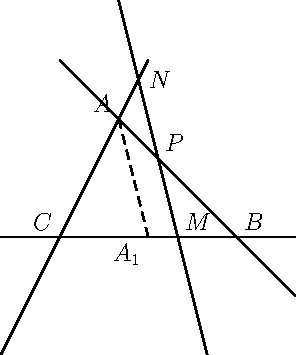
\includegraphics{../images/NDeY-1}$$


Montrons tout d'abord que si $M$, $N$ et $P$ sont alignés, alors $\frac{\overline{MB}}{\overline{MC}}.\frac{\overline{NC}}{\overline{NA}}.\frac{\overline{PA}}
{\overline{PB}}=1$ $(*)$.

On suppose donc que $M$, $N$ et $P$ sont alignés et on note $(\Delta)$ la droite contenant $M$, $N$ et $P$.

\begin{itemize}
\item[\textbf{1ère solution.}] Soit $A_1$ le projeté de $A$ sur la droite $(BC)$ parallèlement à la droite $(\Delta)$. D'après le théorème de \textsc{Thales}, on a

$$\frac{\overline{NC}}{\overline{NA}}=\frac{\overline{MC}}{\overline{MA_1}}\;\mbox{et}\;
\frac{\overline{PA}}{\overline{PB}}=\frac{\overline{MA_1}}{\overline{MB}},$$

et donc,

$$\frac{\overline{MB}}{\overline{MC}}.\frac{\overline{NC}}{\overline{NA}}.\frac{\overline{PA}}
{\overline{PB}}=\frac{\overline{MB}}{\overline{MC}}.\frac{\overline{MC}}{\overline{MA_1}}.\frac{\overline{MA_1}}
{\overline{MB}}=1.$$

\item[\textbf{2ème solution.}] Soit $h_1$ l'homothétie de centre $M$ et de rapport $k_1=\frac{\overline{MB}}{\overline{MC}}$, de sorte que $h_1(C)=B$. Soit $h_2$ l'homothétie de centre $N$ et de rapport $k_2=\frac{\overline{NC}}{\overline{NA}}$, de sorte que $h_2(A)=C$.

Maintenant, le produit $k_1k_2$ peut-il être égal à $1$~?~Si c'était le cas, on aurait $\frac{\overline{MB}}{\overline{MC}}\frac{\overline{NC}}{\overline{NA}}=1$ et donc, $\frac{\overline{MB}}{\overline{MC}}=\frac{\overline{NA}}{\overline{NC}}$. La réciproque du théorème de \textsc{Thales} permettrait alors d'affirmer que $(MN)$ et $(AB)$ sont parallèles, ce qui n'est pas. Donc, $k_1k_2\neq1$ et d'après l'exercice \ref{exo:suprou7bis}, $h_1\circ h_2$ est une homothétie. Puisque $h_1\circ h_2$ transforme $A$ en $B$, son centre est sur la droite $(AB)$. Mais d'autre part, son centre est sur la droite des centres $(MN)$. Finalement, le centre de $h_1\circ h_2$ est le point d'intersection de $(MN)$ et $(AB)$, c'est-à-dire le point $P$.

Mais alors, le rapport de $h_1\circ h_2$ vaut également $\frac{\overline{PB}}{\overline{PA}}$. Ainsi, 
$\frac{\overline{MB}}{\overline{MC}}\frac{\overline{NC}}{\overline{NA}}=\frac{\overline{PB}}{\overline{PA}}$ et finalement, $\frac{\overline{MB}}{\overline{MC}}\frac{\overline{NC}}{\overline{NA}}\frac{\overline{PA}}{\overline{PB}}=1$.

\item[\textbf{3ème solution.}] On se place dans le repère $\mathcal{R}=(A,\overrightarrow{AB},\overrightarrow{AC})$. Dans ce repère, les coordonnées des différents points sont~:~$A(0,0)$, $B(1,0)$, $C(0,1)$, $M(m,1-m)$, $N(0,n)$ et $P(p,0)$ où $m$, $n$ et $p$ sont distincts de $0$ et de $1$.

Les coordonnées de $\overrightarrow{MB}$ sont $(1-m,m-1)$ et celles de $\overrightarrow{MC}$ sont $(-m,m)$. Par suite, $m\overrightarrow{MB}=(m-1)\overrightarrow{MC}$ et finalement, $\frac{\overline{MB}}{\overline{MC}}=\frac{m-1}{m}$. On trouve de même $\frac{\overline{NC}}{\overline{NA}}=\frac{n-1}{n}$ et $\frac{\overline{PA}}{\overline{PB}}=\frac{p}{p-1}$. Finalement,

$$\frac{\overline{MB}}{\overline{MC}}\frac{\overline{NC}}{\overline{NA}}\frac{\overline{PA}}{\overline{PB}}=
\frac{(m-1)(n-1)p}{mn(p-1)}.$$

Maintenant,

\begin{align*}
M,\;N\;\mbox{et}\;P\;\mbox{alignés}\;&\Leftrightarrow
\left|
\begin{array}{cc}
-m&p-m\\
m+n-1&m-1
\end{array}
\right|
\Leftrightarrow-m(m-1)-(p-m)(m+n-1)=0\\
 &\Leftrightarrow-pm-pn+p+mn=0\Leftrightarrow mn=p(m+n-1)\Leftrightarrow mn\\
 &=-p(m-1)(n-1)+pmn\Leftrightarrow p(m-1)(n-1)=mn(p-1)\\
 &\Leftrightarrow\frac{(m-1)(n-1)p}{mn(p-1)}=1
\end{align*}

\end{itemize}

Montrons maintenant que si $\frac{\overline{MB}}{\overline{MC}}\frac{\overline{NC}}{\overline{NA}}\frac{\overline{PA}}{\overline{PB}}=1$, alors les points $M$, $N$ et $P$ sont alignés. Pour cela, vérifions tout d'abord que $(MN)$ n'est pas parallèle à $(AB)$. Dans le cas contraire, le théorème de \textsc{Thales} fournirait $\frac{\overline{MB}}{\overline{MC}}\frac{\overline{NC}}{\overline{NA}}=1$ et donc  $\frac{\overline{PA}}{\overline{PB}}=1$, puis $\overline{PA}=\overline{PB}$ et finalement $\overline{AB}=0$, ce qui n'est pas.

Par suite, la droite $(MN)$ coupe la droite $(AB)$ en un point $P_1$ vérifiant d'après le début de l'exercice

$\frac{\overline{MB}}{\overline{MC}}\frac{\overline{NC}}{\overline{NA}}\frac{\overline{P_1A}}{\overline{P_1B}}=1$. On en déduit que $\frac{\overline{P_1A}}{\overline{P_1B}}=\frac{\overline{PA}}{\overline{PB}}$. Notons $k$ la valeur commune de ce rapport.

On a déjà que $k\neq1$, ou encore $1-k\neq0$. Par suite, $P_1=\mbox{bar}\{A(1),B(-k)\}=P$, ce qui montre que les points $M$, $N$ et $P$ sont alignés.
}
}
